%% Alban Kraus
%% © 2016 École nationale des sciences géographiques
%% 6-8 avenue Blaise Pascal - Champs-sur-Marne
%% 77455 MARNE-LA-VALLÉE CEDEX 2

\documentclass[a4paper, oneside, twocolumn, 12pt]{report}

% Directories
\newcommand\fragment{fragment}
\newcommand\data{data}
\newcommand\appendices{appendix}

% French typesetting
\usepackage[utf8]{inputenc}
\usepackage[T1]{fontenc}
\usepackage[english, french]{babel}
\usepackage{numprint}
\usepackage{lmodern}

% Meta-data
\usepackage{color}
\usepackage[
  hyperindex=true,
  bookmarks=true,
  baseurl={https://github.com/alkra/MPIMP},
  pdftitle={Rapport des TP de parallélisation},
  pdfauthor={Alban Kraus},
  pdfsubject={Parallélisation -- mars 2016},
  pdfproducer={École nationale des sciences géographiques -- 6-8 avenue Blaise Pascal - Champs-sur-Marne -- 77455 MARNE-LA-VALLÉE CEDEX 2},
  pdflang=fr-FR
]{hyperref}

\title{Rapport des TP de parallélisation}
\author{Alban Kraus}
\date{23 mars 2016}

% Headings customization
\usepackage{titlesec}

\newcounter{question}[chapter]
\renewcommand\thesubsection{Q.~\arabic{question}}
\titleformat{\subsection}[hang]{\stepcounter{question}\normalfont\large\bfseries}{Question~\arabic{question}}{0.7em}{}{}
\newcommand\question{\subsection{\null}}
\titleformat{\chapter}[display]{\normalfont\huge\bfseries\centering}{TP~\thechapter}{20pt}{\Huge}

% Other packages (style - maths - graphics)
\usepackage{framed}
\usepackage{longtable}
\usepackage{tabularx}
\usepackage{array}
\usepackage{amsmath}
\usepackage[scientific-notation=true]{siunitx}
\usepackage{pgfplots}
\pgfplotsset{compat=1.11}
\pgfplotsset{width=7.5cm}
\usepackage{tikz}
\usepackage{transparent}
\usepackage{graphicx}
\usepackage{eso-pic}

% First page's overlay
\newcommand\BackgroundPic{%
  \put(0, 0){%
    \parbox[b][\paperheight]{\textwidth}{%
      \transparent{0.3}%
      \vfill%
      \centering%
      \lstset{%
        basicstyle=\footnotesize,
        showspaces=false
      }%
      \lstinputlisting[language=C, firstline=217, lastline=391, nolol
      ]{\fragment/mandel.c}%
      \vfill%
    }%
  }%
}

% Code
\usepackage{listings}
\definecolor{comments}{gray}{0.7}
\definecolor{keywords}{rgb}{0.1, 0.1, 0.9}
\definecolor{strings}{rgb}{0.8, 0.05, 0.7}
\lstset{
  commentstyle=\color{comments}\rmfamily,
  keepspaces=true,
  keywordstyle=\color{keywords},
  stringstyle=\color{strings}
}

\usepackage[french, longend, ruled]{algorithm2e}
% Constantes
\SetKwData{MASTER}{MAÎTRE}

% Entrées / sorties
\SetKwInput{Variables}{Variables locales}
\SetKwData{H}{h}
\SetKwData{W}{w}
\SetKwData{P}{nproc}
\SetKwData{Rank}{rank}
\SetKwData{Hlocal}{h\_local}
\SetKwData{Ima}{ima}
\SetKwData{Pima}{pima}
\SetKwData{Xmin}{xmin}
\SetKwData{Xmax}{xmax}
\SetKwData{Ymin}{ymin}
\SetKwData{Ymax}{ymax}
\SetKwData{Xincr}{xincr}
\SetKwData{Yincr}{yincr}
\SetKwData{Filtre}{filtre}
\SetKwData{Niter}{nbiter}
\SetKwData{R}{r}

% fonctions C
\SetKwFunction{sizeof}{sizeof}
\SetKwFunction{malloc}{malloc}

% fonctions MPI
\SetKwData{CommWorld}{MPI\_COMM\_WORLD}
\SetKwData{Char}{MPI\_CHAR}
\SetKwData{Int}{MPI\_INT}
\SetKwFunction{Recv}{MPI\_Recv}
\SetKwFunction{Send}{MPI\_Send}
\SetKwFunction{Bcast}{MPI\_Bcast}
\SetKwFunction{Scatter}{MPI\_Scatter}
\SetKwFunction{Gather}{MPI\_Gather}
\SetKwData{AnySource}{MPI\_ANY\_SOURCE}
\SetKwFunction{Probe}{MPI\_Probe}
\SetKwData{Source}{MPI\_SOURCE}
\SetKwData{Exchange}{TAG\_LINE\_EXCHANGE}

% Style
\DontPrintSemicolon









%%%%%%%%%%%%
% DOCUMENT %
%%%%%%%%%%%%


\begin{document}

% Title page
\twocolumn[
\begin{@twocolumnfalse}
  \newlength\ensg
\settowidth\ensg{\small 6-8 avenue Blaise Pascal -- Champs-sur-Marne}

\begin{titlepage}

  % Background picture
  \AddToShipoutPicture*{\BackgroundPic}

  % ENSG
  \begin{flushright}
    \begin{tabular}{p{\ensg} p{0.25\textwidth}}
      {%
      \small
      ~\newline
      École nationale des sciences géographiques

      6-8 avenue Blaise Pascal -- Champs-sur-Marne\newline
      77455 MARNE-LA-VALLÉE CEDEX 2
      } & \raisebox{-0.9\height}[0pt][0.8\height]{%
          
\includegraphics[width=0.25\textwidth]{\fragment/logo_ensg}%
          } \\
    \end{tabular}
  \end{flushright}

  % Titles
  \begin{center}
    \vskip 0.1\textheight

    \begin{framed}
      \bigskip

      \Huge\sffamily\bfseries
      Rapport des travaux pratiques

      \bigskip

      \LARGE\rmfamily\mdseries
      Cours de parallélisation

      de Ahmad \bsc{Audi}

      \bigskip
    \end{framed}

    \vskip 0.1\textheight

    \bfseries\Large
    Alban Kraus
    
    \smallskip

    \normalsize\mdseries
    Cycle ingénieur, promotion 2013

    \vskip 0.18\textheight

    23 mars 2016
  \end{center}
\end{titlepage}


%%% Local Variables:
%%% mode: latex
%%% TeX-master: "rapport"
%%% End:

\end{@twocolumnfalse}
]

\clearpage

% Copyright notice
\thispagestyle{empty}
\twocolumn[
\begin{@twocolumnfalse}
  \vskip 0.8\textheight

  \begin{minipage}{\textwidth}
  \centering\footnotesize
  Cette œuvre est protégée en France et dans d'autre pays.
  
  \bigskip

  
\includegraphics{\fragment/CC-BY}
    
  \bigskip

  Vous pouvez réutiliser cette œuvre selon les termes de la licence

  \href{https://creativecommons.org/licenses/by/3.0/deed.fr}{%
    Creative commons -- attribution 3.0 non transposé}
\end{minipage}


%%% Local Variables:
%%% mode: latex
%%% TeX-master: "../rapport"
%%% End:

\end{@twocolumnfalse}
]

\clearpage

\tableofcontents


% TP 1

\chapter{Ensemble de Mandelbrot}

\loop\ifnum\arabic{question}<5
\input{mandelbrot/question-\arabic{question}}
\repeat

% TP 2

\chapter{Convolution}

%% Alban Kraus
%% © 2016 École nationale des sciences géographiques
%% 6-8 avenue Blaise Pascal - Champs-sur-Marne
%% 77455 MARNE-LA-VALLÉE CEDEX 2

\section{Questions liminaires}

\subsubsection{La fonction convolution}

\begin{quotation}
  Dans la fonction \texttt{con\-vo\-lu\-tion(\-)}, pourquoi doit-on
  préparer un tampon intermédiaire au lieu de faire le calcul
  directement sur l'image ?
\end{quotation}

Le filtre s'applique à plusieurs pixels de l'image \emph{originale}
(ou de la convolution $i-1$). Si on fait le calcul directement sur
l'image (convolution $i$), il y aura au moins un de ces pixels qui
aura été altéré par le calcul précédent.

On a alors besoin de deux tampons : l'un contient l'image originale,
et l'autre l'image convoluée. À la fin du calcul, on remplace l'image
originale par l'image convoluée, qui sera l'image originale de la
prochaine convolution.


\subsubsection{Parallélisation de l'algorithme}

\begin{quotation}
  Quelles sont les séquences parallélisables de l'algorithme ?
\end{quotation}

Le calcul de la convolution ne dépend que de l'image originale : il
peut donc \^etre parallélisé. Autrement dit, le calcul de chaque pixel
est indépendant.

L'application du filtre ne peut pas \^etre parallélisée en règle
générale.

De plus, la composition des convolutions ne peut pas \^etre
parallélisée, car chacune dépend de la précédente.



\subsubsection{Équilibrage de charge}

\begin{quotation}
  Sachant que la taille du noyau $k$ de convolution est $3 \times 3$
  pixels, quelle est la complexité théorique du calcul d'un pixel de
  $I * k$ ? Quel type d'équilibrage de charge doit-on prévoir entre
  les processeurs ?
\end{quotation}

Pour chaque pixel, l'application du filtre se fait en temps constant
(ne dépend que de la taille du filtre). On peut donc appliquer une
répartition statique de charge.


\subsubsection{Découpage}

\begin{quotation}
  Quel découpage (répartition des données entre processeurs) est
  naturel dans ce contexte ?
\end{quotation}

Afin de minimiser les communications entre processus, et aussi parce
qu'il est plus simple à mettre en place, nous allons réaliser un
découpage en \emph{lignes}.


\subsubsection{Problèmes aux bords}

\begin{quotation}
  Quel problème (au bord des blocs de l'image) survient lors de
  l'itération de l'opération de convolution ?
\end{quotation}

Lors du calcul d'un bloc de l'image, chaque processus aura besoin de
la dernière ligne du processus précédent et de la première du suivant
pour calculer sa première ligne et sa dernière.

Chaque processus doit ainsi communiquer sa première ligne au processus
précédent et sa dernière ligne au processus suivant.


\subsubsection{Pseudo-code}

\begin{quotation}
  Implémenter un algorithme parallèle avec des envois bloquants de
  message.
\end{quotation}

\begin{algorithm}[t]
  \caption{Lecture de l'image}
  \label{alg:convol:stat:file}
  \Donnees{\;
    \begin{tabular}{l @{ : } l}
      \Rank & rang du processus (connu)\\
    \end{tabular}
  }

  \Variables{\;
    \begin{tabularx}{\linewidth}{l @{ : } X}
      $params$ & tableau [2] contenant les tailles des images\\
    \end{tabularx}
  }

  \Res{\;
    \begin{tabular}{l @{ : } l}
      \R & fichier image\\
      \H & hauteur de l'image\\
      \W & largeur de l'image\\
    \end{tabular}
  }

  \Deb{%
    \Si{\Rank == \MASTER}{%
      Lecture du fichier\;
      Récupération de $params$\;
    }

    \tcp{Envoi des paramètres}
    \hangindent=\skiptext\hangafter=1
    \Bcast{$params$, 2, \Int, \MASTER, \CommWorld}\;
    \H = $params$[0]\;
    \W = $params$[1]\;
  }
\end{algorithm}

Les algorithmes \ref{alg:convol:stat:file} et
\ref{alg:convol:stat:mem} ne nécessitent que peu d'explications. Le
processus maître lit l'image et l'envoie à ses esclaves. La fonction
\texttt{MPI\_Scatter} se charge de répartir statiquement la charge de
travail entre les processus esclaves.

Néanmoins, comme établi à la question précédente, cet envoi ne
concerne que les lignes propres au processus en question. Les échanges
de lignes se déroulent dans l'algorithme \ref{alg:convol:stat:calc}.

\begin{algorithm*}
  \caption{Allocation de la mémoire}
  \label{alg:convol:stat:mem}

  \Donnees{\R, \H, \W, \Rank\;
    \begin{tabular}{l @{ : } l}
      \P & nombre de processus (connu)\\
    \end{tabular}
  }

  \Res{\;
    \begin{tabularx}{\linewidth}{l @{ : } X}
      \Hlocal & hauteur d'un bloc\\
      \Ima & pointeur vers le début de l'image\\
    \end{tabularx}
  }

  \Deb{
    \hangindent=\skiptext\hangafter=1
    \Hlocal = \H / \P \\
    + (\Rank > 0 ? 1 : 0)\\
    + (\Rank < \P-1 ? 1 : 0)\;

    \uSi{\Rank == \MASTER}{
      \Ima = \R.data;
    }
    \Sinon{
      \hangindent=\skiptext\hangafter=1
      \Ima = \malloc{\Hlocal * \W * \sizeof{unsigned char}}\;
      Test de l'allocation\;
    }

    \hangindent=\skiptext\hangafter=1
    \Scatter{
      \Ima, \mbox{\W * \H / \P, \Char},
      \mbox{\Ima + (\Rank > 0 ? \W : 0)},
      \mbox{\W * \H / \P}, \Char, \MASTER, \CommWorld
    }\;
  }
\end{algorithm*}

Chaque processus différent du premier commence par envoyer sa deuxième
ligne au précédent. Pour éviter un blocage perpétuel, le deuxième
\texttt{if} doit commencer par la réception de la dernière
ligne. Explications dans le tableau \ref{tab:convol:stat:bloquant}.

Une fois l'échange de lignes effectué, le travail peut
commencer. Entre chaque application du filtre, les processus échangent
à nouveau leurs lignes extrêmes, car elles ont été modifiées.

À la fin du calcul, tous les processus envoient leur résultat sans la
première ni la dernière ligne, et \texttt{MPI\_Gather} se charge de
refabriquer l'image finale.

\begin{table*}
  \centering
  \begin{tabularx}{\linewidth}{X X X X}
    Processus 0 & Processus 1 & Processus 2 & Processus 3\\
    \hline
    Recv(1) \hfill $\leftarrow$  & Send(0)   & Send(1)     & Send(2)\\
    Send(1) \hfill $\rightarrow$ & Recv(0)   & Send(1)     & Send(2)\\
    \hline
    (travail) & Recv(2) \hfill $\leftarrow$  & Send(1)   & Send(2)\\
              & Send(2) \hfill $\rightarrow$ & Recv(1)   & Send(2)\\
    \hline
              & (travail) & Recv(3) \hfill $\leftarrow$  & Send(2)\\
              &           & Send(3) \hfill $\rightarrow$ & Recv(3)\\
    \hline
              &           & (travail)             & (travail)\\
  \end{tabularx}
  \caption{Échange bloquant des lignes}
  \label{tab:convol:stat:bloquant}
\end{table*}

\begin{algorithm*}
  \caption{Calcul et envoi du résultat}
  \label{alg:convol:stat:calc}

  \Donnees{\Ima, \W, \H, \Hlocal, \Rank, \P\;
    \begin{tabular}{l @{ : } l}
      \Filtre & numéro du filtre (commande)\\
      \Niter & nombre d'itérations (commande)\\
    \end{tabular}
  }

  \Variables{\;
    \begin{tabular}{l @{ : } l}
      $status$ & état de la requête\\
      $i$ & itération courante\\
    \end{tabular}
  }

  \Deb{%
    \Pour{$i$ de 0 à \Niter} {
      \tcp{Communications avec le processus précédent}
      \Si{\Rank > 0}{
        \Send{\Ima + \W, \W, \Char, \Rank-1, \Exchange, \CommWorld}\;
        \Recv{\Ima, \W, \Char, \Rank-1, \Exchange, \CommWorld,
          \&$status$}\;
      }

      \tcp{Communications avec le processus suivant}
      \Si{\Rank < \P-1}{
        \Recv{%
          \mbox{\Ima + (\Hlocal-1) * \W},
          \W, \Char, \Rank+1, \Exchange, \CommWorld, \&$status$
        }\;
        \Send{%
          \mbox{\Ima + (\Hlocal-2) * \W},
          \W, \Char, \Rank+1, \Exchange, \CommWorld
        }\;
      }

      calcul(\Filtre, \Ima, \Hlocal, \W)\;
    }

    \Gather{%
      \mbox{\Ima+\W},
      \mbox{\W * \H / \P}, \Char, \Ima,
      \mbox{\W * \H / \P}, \Char, \MASTER, \CommWorld
    }\;

    \Si{\Rank == \MASTER}{%
      Enregistrement de \Ima\;
    }
  }
\end{algorithm*}

\subsubsection{Analyse des performances}

Les tests ont été effectués sur l'image Albert-Einstein.ras en figure
\ref{fig:convol:einstein}, dont la provenance est douteuse. Cette
image a pour dimensions $1200 \times 1000$.

\begin{figure}
  \centering
  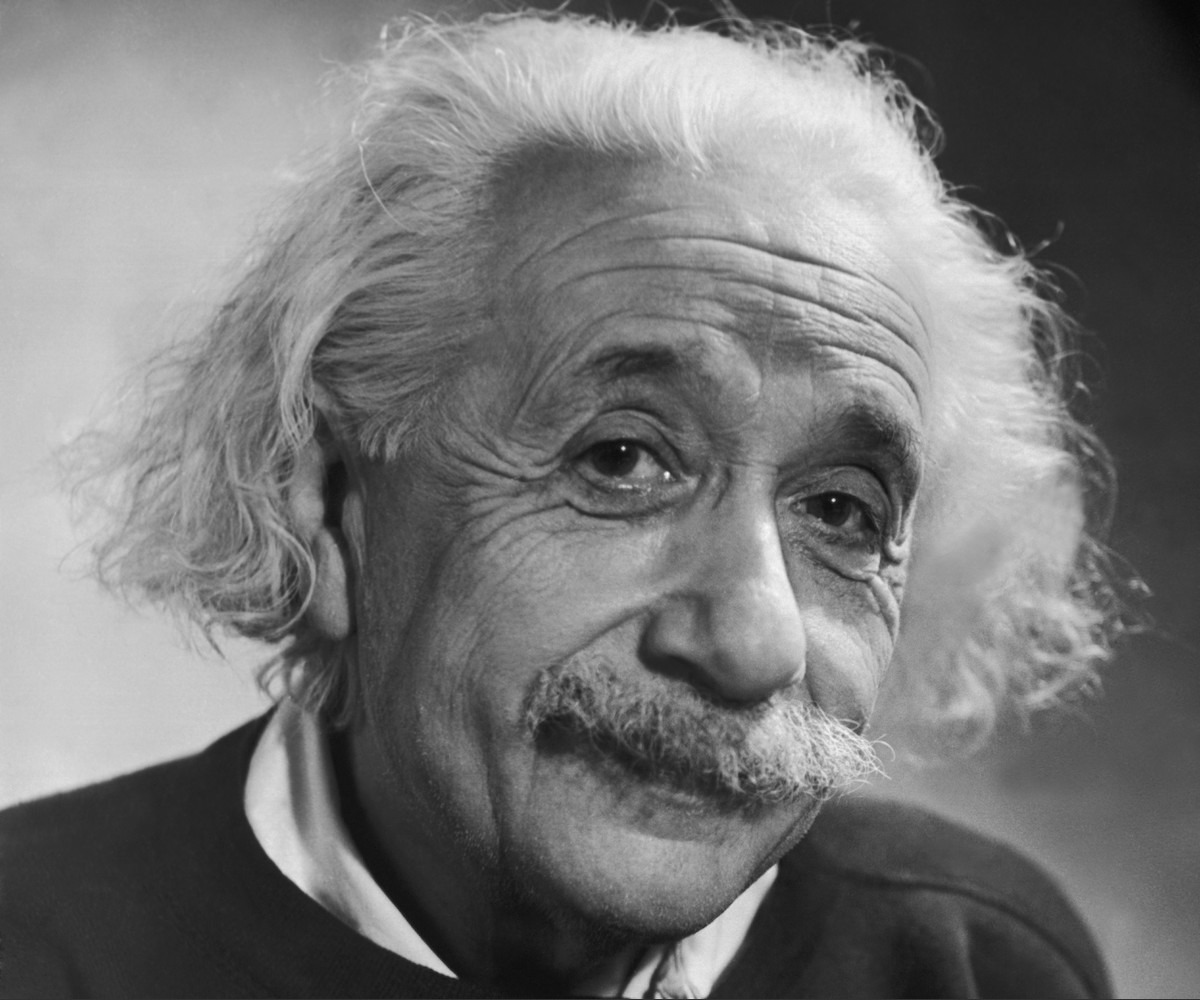
\includegraphics[width=\linewidth]{\fragment/Albert-Einstein}
  \caption{L'image de test}
  \label{fig:convol:einstein}
\end{figure}

Dans la figure \ref{fig:convol:iter}, on s'intéresse aux performances
de calcul en fonction du nombre d'itérations. Le filtre 4 est beaucoup
plus long à appliquer que les autres ; il fait donc l'objet d'un
diagramme séparé.

\paragraph{Le filtre 4}
Toutes les courbes sont linéaires et s'intersectent en $(0, 0)$. On
peut donc en lire la pente aisément : avec six machines, le filtre 2
a une pente de 4 secondes par millier d'itérations, et le filtre 4 de
120 secondes par millier d'itérations. La pente du filtre 4 est donc
trente fois plus grande que celle des autres filtres. Le tri des
valeurs pour en extraire la médiane peut être une source de calculs
supplémentaires ; pour valider cette hypothèse, il serait nécessaire
d'examiner le code assembleur et compter les opérations, ce qui me
paraît trop compliqué pour le cadre de ce TP.

\begin{figure}
  \centering

  \begin{tikzpicture}
    \begin{axis}[
      xlabel={Nombre d'itérations},
      ylabel={Temps de calcul (s)},
      legend style={
        at={(0.5,1)},
        anchor=south
      }
      ]

      \addplot[red, dashed] table [x index=3, y index=4,
      col sep=semicolon, header=false]{%
        \data/convol-iter-1-4.csv%
      };

      \addplot[red] table [x index=3, y index=4,
      col sep=semicolon, header=false]{%
        \data/convol-iter-6-4.csv%
      };

      \legend{filtre 4 (1 machine), filtre 4 (6 machines)}
    \end{axis}
  \end{tikzpicture}

  \begin{tikzpicture}
    \begin{axis}[
      xlabel={Nombre d'itérations},
      ylabel={Temps de calcul (s)},
      legend style={
        at={(0.5,1)},
        anchor=south
      }
      ]
      \addplot[black, dashed] table [x index=3, y index=4,
      col sep=semicolon, header=false]{%
        \data/convol-iter-1-0.csv%
      };

      \addplot[blue, dashed] table [x index=3, y index=4,
      col sep=semicolon, header=false]{%
        \data/convol-iter-1-2.csv%
      };

      \addplot[black] table [x index=3, y index=4,
      col sep=semicolon, header=false]{%
        \data/convol-iter-6-0.csv%
      };

      \addplot[blue] table [x index=3, y index=4,
      col sep=semicolon, header=false]{%
        \data/convol-iter-6-2.csv%
      };

      \legend{filtre 0 (1 machine), filtre 2 (1 machine), filtre 0 (6
        machines), filtre 2 (6 machines)}
    \end{axis}
  \end{tikzpicture}

  \caption{Temps de calcul en fonction du nombre d'itérations ; sur 1 ou 6 machines}
  \label{fig:convol:iter}
\end{figure}

Toutes les courbes concordent : le temps de calcul est linéaire par
rapport au nombre d'itérations. En effet, l'application du filtre se
fait en temps constant. Les écarts observés lorsqu'une seule machine
est utilisée doivent être expliqués par le fait que j'utilisais cette
machine pour taper mon rapport : tous les processus n'étaient donc pas
entièrement consacrés au calcul. Cela dit, cette hypothèse est à
tempérer, puisque ces mesures ont été acquises avec deux processus sur
une machine disposant de huit cœurs...


\begin{figure}
  \centering

  \begin{tikzpicture}
    \begin{axis}[
      xlabel={Nombre de processus},
      ylabel={Temps de calcul (s)},
      legend style={
        at={(0.5,1)},
        anchor=south
      }
      ]
      \addplot[black, dashed] table [x index=1, y index=4,
      col sep=semicolon, header=false]{%
        \data/convol-proc-1-0.csv%
      };

      \addplot[red, dashed] table [x index=1, y index=4,
      col sep=semicolon, header=false]{%
        \data/convol-proc-1-4.csv%
      };

      \addplot[black] table [x index=1, y index=4,
      col sep=semicolon, header=false]{%
        \data/convol-proc-6-0.csv%
      };

      \addplot[red] table [x index=1, y index=4,
      col sep=semicolon, header=false]{%
        \data/convol-proc-6-4.csv%
      };

      \legend{filtre 0 (1 machine), filtre 4 (1 machine), filtre 0 (6
        machines), filtre 4 (6 machines)}
    \end{axis}
  \end{tikzpicture}

  \caption{Temps de calcul en fonction du nombre de processus ; sur 1
    ou 6 machines}
  \label{fig:convol:proc}
\end{figure}

\paragraph{Nombre de processus}
Les courbes de la figure \ref{fig:convol:proc} ont la même forme que
celles obtenues au TP précédent. L'interprétation en est identique.

%%% Local Variables:
%%% mode: latex
%%% TeX-master: "../rapport"
%%% End:


% TP 3

\chapter{OpenMP}

%% Alban Kraus
%% © 2016 École nationale des sciences géographiques
%% 6-8 avenue Blaise Pascal - Champs-sur-Marne
%% 77455 MARNE-LA-VALLÉE CEDEX 2

\lstset{%
  basicstyle=\footnotesize,
}%

\section{Questions}

\subsection{Nombre de cœurs disponibles}

\begin{quotation}
  Vérifiez à l'aide de la commande \texttt{cat /proc/cpuinfo} le
  nombre de cœurs disponible sur votre machine.
\end{quotation}

Cette commande affiche les statistiques de \emph{huit} cœurs de
calcul~; il faut noter que l'hyperthreading est activé, donc il n'y a
en réalité qu'un processeur à quatre cœurs.

\subsection[Premier programme]{1\textsuperscript{er} programme}

\begin{quotation}
  Utiliser un des programmes du cours pour tester votre
  environnement. N'oubliez pas de positionner la variable
  \texttt{OMP\_NUM\_THREADS} !
\end{quotation}

\subsection{Calcul de fractales}

\begin{quotation}
  Le fichier \texttt{mandel.c} contient le code source d'un programme
  qui calcule les valeurs de l'espace de Mandelbrot.

  Parallélisez ce programme avec OpenMP, puis exécutez-le avec des
  équilibrages de charges statiques et dynamiques et avec différentes
  valeurs de taille de bloc.
\end{quotation}

Pour paralléliser ce calcul, on utilise l'interface de compilation
d'OpenMP (directives \texttt{\#pragma omp} et compilation avec
\texttt{gcc -fopenmp}). En particulier, on ajoute une première ligne
et un bloc d'accolades pour délimiter la zone à paralléliser, et on
parallélise une boucle \texttt{for}.

L'algorithme séquentiel a dû être légèrement modifié pour faire en
sorte que les modifications des variables locales ne soient pas
écrasées par les processus. Une variable \emph{privée} sera propre à
chaque processus, et chaque processus peut avoir une valeur différente
pour cette variable. Le code est affiché au listing
\ref{lst:omp:mandel:seq}.

\lstinputlisting[float=*, language=C, firstline=269,
lastline=283, caption=Code de Mandelbrot modifié pour OpenMP,
label=lst:omp:mandel:seq]{\fragment/mp-seq-mandel.c}

On peut même combiner OpenMP et OpenMPI, de manière à paralléliser
chaque processus. Par manque de temps, aucune mesure n'a pu être
prise, ce qui est bien dommage : il faudrait mesurer la différence (ou
plutôt, selon ma conjecture, l'absence de différence) entre six
processus non threadés, un processus avec six threads, et six
processus avec six threads sur une seule machine ; puis la différence
entre six processus non threadés et six processus threadés sur six
machines à huit cœurs. Le code est présenté au listing
\ref{lst:omp:mandel:stat}.

\lstinputlisting[float=*, language=C, firstline=304,
  lastline=322,
  caption=Code statique de Mandelbrot modifié pour OpenMP,
  label=lst:omp:mandel:stat]{\fragment/mp-stat-mandel.c}

Dans ce code, les lignes à générer sont partagées entre les processus,
puis chaque processus les partage à nouveau entre ses fils d'exécution.



\subsection{Convolution}

\begin{quotation}
  Le fichier \texttt{convol.c} contient le code source d'un programme
  qui applique des opérateurs de convolution à des images.

  Parallélisez ce programme avec OpenMP, puis exécutez-le avec des
  équilibrages de charge statiques et dynamiques et avec différentes
  valeurs de taille de bloc.
\end{quotation}

Le code modifié est présenté au listing \ref{lst:omp:convol:seq}. De
même que dans le TP précédent, c'est la boucle qui applique le filtre
qui est parallélisée. Sans raison véritable, j'ai parallélisé aussi la
boucle réalisant les copies de mémoire-tampon.

\lstinputlisting[float=*, language=C, linerange={255-267, 274-278},
caption=Code de convolution modifié pour OpenMP,
label=lst:omp:convol:seq
]{\fragment/mp-seq-convol.c}

%%% Local Variables:
%%% mode: latex
%%% TeX-master: "../rapport"
%%% End:


% Annexes
\appendix
\titleformat{\chapter}[display]{\normalfont\huge\bfseries\centering}{Annexe~\thechapter}{20pt}{\Huge}


\chapter{Guide d'installation}
\label{app:install}

Le code du TP est versionné à l'aide du système Git. Il est réparti
sur plusieurs branches, qui ne sont pas destinées à être fusionnées
(voir l'annexe \ref{app:git}). Ainsi, la récupération de toutes les
branches est indispensable.

\section{Prérequis}

\subsubsection{Pour le code}

\paragraph{Linux}
Les programmes sont écrits en C, et conçus pour fonctionner sur un
système \emph{à la Unix} (GNU/Linux, BSD, Mac, ...). Windows n'est
officiellement pas supporté ; toutefois, si vous avez les
connaissances requises (adapter les chemins de fichier, installer
les programmes \texttt{GNU}, \texttt{sed}, \texttt{bash}, déboguer les
\texttt{Makefile}s), le projet devrait fonctionner correctement.

\paragraph{GCC}
Il vous faut un compilateur C. Nous utilisons \texttt{gcc}. Si vous
souhaitez utiliser un autre compilateur, il vous faudra adapter les
\texttt{Makefile}s. (voir l'annexe \ref{app:Makefiles}).

\paragraph{OpenMPI}
OpenMPI comprend une bibliothèque C, à installer dans le répertoire
correspondant de votre compilateur, et une collection de binaires
(notamment le pseudo-compilateur \texttt{mpicc} et
\texttt{mpirun}). Les distributions GNU/Linux de type Debian les
distribuent dans les paquets \texttt{libopenmpi-dev} et
\texttt{openmpi-bin}.

\paragraph{OpenMP}
Assurez-vous d'utiliser un com\-pi\-la\-teur compatible avec les
directives OpenMP. Il n'y a rien à installer.

\paragraph{Make}
GNU \texttt{make} est un programme permettant d'automatiser la
compilation (voir annexe \ref{app:Makefiles}). Le paquet Debian a pour
nom \texttt{make}.

\paragraph{Git}
Git est un système de gestion de versions distribué. Pour plus de
détails quant à son utilité pour le projet, reportez-vous à l'annexe
\ref{app:git}.

\paragraph{openssh}
\texttt{openssh} permet d'ouvrir un shell sécurisé sur une machine
distante. Nous en avons besoin pour lancer des programmes MPI sur
plusieurs machines. (voir la section \ref{sec:installation:machines})

\paragraph{bash}
Nos scripts d'automatisation sont à exécuter dans le
\emph{\textbf{B}ourne-\textbf{a}gain \textbf{sh}ell}. \texttt{bash}
devrait être installé sur la plupart des distributions GNU/Linux et
Mac.

\subsubsection{Pour le rapport}

Le rapport est rédigé en \LaTeX. Si vous souhaitez le recompiler, vous
aurez besoin des paquets cités ci-après.


\paragraph{GNU/Linux, Make, Git} \emph{confere supra}.

\paragraph{pdflatex}
Une distribution \TeX\,/\,\LaTeX\ est composée d'un interpréteur
(respectivement \texttt{[pdf]tex} et \texttt{[pdf]latex}) générant un
fichier au format \emph{\textbf{d}e\textbf{v}ice
  \textbf{i}ndependant}, destiné à être compris par toutes les
imprimantes, ou directement dans le \emph{\textbf{p}ortable
  \textbf{d}ocument \textbf{f}ormat} (PDF) qui est mieux adapté à une
lecture dématérialisée ; et d'un grand nombre de paquets qui
enrichissent le langage. L'ensemble est distribué sous le nom de \TeX
live sous GNU/Linux, Mac\TeX\ sous Mac, et Mik\TeX\ sous Windows. Si
vous êtes sous Debian, vous aurez besoin des paquets suivants :
\texttt{texlive-latex-extra}, \texttt{texlive-science}, et
\texttt{texlive-lang-french} ; par le jeu des dépendances, vous
installerez tous les autres paquets nécessaires. Les autres
distributions proposent un moyen d'installer les paquets \LaTeX\ à la
volée.

\section{MPI – Configuration des machines}
\label{sec:installation:machines}

Cette section décrit le script \texttt{init-mpi}.

Le fichier \texttt{hosts} dans les dossiers des sources contient la
liste des machines à utiliser pour lancer les programmes. Il doit y
avoir une adresse IP ou nom de domaine par ligne. Le programme sera
recompilé sur la première machine listée.

Les communications au sein d'un communicateur utilisent des
connections SSH. \emph{Il ne doit pas être demandé de mot de
  passe}. Pour cela, vous avez la possibilité de modifier la
configuration de PAM pour ne pas authentifier la connexion, ou bien
utiliser une authentification à base de clés openssh.

Pour générer une clé, on ouvre un shell sur la première machine, et on
lance la commande \texttt{ssh-keygen -t rsa -b 1024}. Pour la suite de
cette section, il sera considéré que vous avez laissé le nom de
fichier par défaut. Ne pas entrer de mot de passe, tapez \emph{Entrée}
directement aux deux invites.

On génère une clé courte (1024 bits) pour ne pas trop perdre de
temps. Si le système est critique, ou l'utilisation en est prolongée,
augmenter cette valeur.

Le fichier \texttt{id\_rsa} contient la clé par défaut associée à
l'utilisateur.

On ne protège pas la clé par un mot de passe, puisque l'objet de cette
démarche est justement de ne pas avoir à taper de mot de passe.

On va ensuite faire connaître cette clé à toutes nos machines, en
utilisant une boucle \texttt{for} qui épluche le fichier
\texttt{hosts}. Vous êtes encouragé à utiliser le même nom
d'utilisateur sur toutes les machines ; dans le cas contraire, de
nombreux scripts et configuration de ces annexes ne marcheront pas.

\begin{lstlisting}[language=bash]
for host in $(cat hosts)
do
    ssh-copy-id $host
done
\end{lstlisting}

Et on recommance pour toutes les machines. En fait, on peut encapsuler
ces trois commandes dans une boucle \texttt{for} depuis le répertoire
du ficher hosts. Pensez à adapter le dossier de destination.


\section{Récupération des sources}

Les sources sont hébergées en ligne, sur mon GitHub, à l'adresse
\url{https://github.com/alkra/MPIMP}. Pour les télécharger, nous
allons utiliser le client \texttt{git}. Le contenu du dépôt sera copié
dans un sous-dossier MPIMP du dossier courant.

\begin{verbatim}
git clone \
    https://github.com/alkra/MPIMP
\end{verbatim}

Ce n'est pas fini ! Pour l'instant, vous n'avez récupéré que la
branche \emph{master} du dépôt. Vous devez suivre les autres
branches (listing \ref{lst:installation:clone}).

\begin{lstlisting}[float=*, language=bash, caption=Copie du dépôt,
  label=lst:installation:clone]
cd MPIMP
for branch in mpi-master mpi-static mpi-dynamic \
              mp-seq mp-static mp-dynamic
do
    git checkout -b $branch origin/$branch
done
git checkout master
\end{lstlisting}

Voir l'annexe \ref{app:git} pour plus de détails.



\section{Compilation et lancement}

\subsubsection{Programmes séquentiels}

Il suffit de copier (avec \texttt{scp}) le dossier source sur la
machine distante, s'y déplacer, et lancer \texttt{make} suivi de
\texttt{./mandel.akraus}. L'extension de ce fichier exécutable vient
du fait que, dans les conditions du TP, tous les étudiants
travaillaient sur les mêmes machines dans le même dossier : il fallait
donc différentier les exécutables de chacun.

\subsubsection{MPI}

Sur les branches dérivant de \emph{mpi-master} se trouve un script
\texttt{propagate}, décrit en annexe \ref{app:propagate}, qui se
charge de mener à bien la compilation, le lancement, et la
récupération des résultats.

\begin{verbatim}
./propagate --help
./propagate <options>
\end{verbatim}



\section{Nettoyage – todo-list}

Il faut supprimer les fichiers copiés sur toutes les machines
distantes. Vous pouvez faire une boucle \texttt{for} sur le contenu du
fichier hosts.

Sur la première machine, faire un \texttt{make clean} pour supprimer
les exécutables et fichiers de compilation. Supprimez aussi les
fichiers de résultat, ainsi que l'ensemble des sources.

Enlevez les $n$ dernières lignes des fichiers
\texttt{\string~/.ssh/authorized\_keys} de toutes les machines, où $n$
est le nombre de lignes du fichier hosts. Chaque ligne de ceux-là
représente la clé d'un des hôtes. Enfin, sur chaque machine, supprimez
\texttt{\string~/.ssh/id\_rsa} et \texttt{\string~/.ssh/id\_rsa.pub}.




\section{Compiler le rapport}

D'abord, assurez-vous avec un \texttt{git status} que vous n'avez
aucune modification détectée. Si des noms de fichier rouges
apparaissent avant la section \emph{Fichiers non suivis (Untracked
  files)}, validez-les, ou annulez-les avec \texttt{git checkout --
  <fichier>}.

Déplacez-vous ensuite dans le sous-dossier \texttt{Rapport} de la
branche \emph{master}, et lancez \texttt{make}. Cela va générer un
grand nombre de fichiers csv dans \texttt{data}, que vous pourrez
supprimer avec un \texttt{make clean}, afficher beaucoup de lignes sur
votre terminal, et enfin générer un fichier \texttt{rapport.pdf}.

%%% Local Variables:
%%% mode: latex
%%% TeX-master: "../rapport"
%%% End:


\newenvironment{git}{
  \bigskip
  \noindent%
  \begin{tikzpicture}[scale=0.9]%
}{%
  \end{tikzpicture}
  \bigskip
}

\gdef\ccommit[#1](#2,#3)#4{
  (#2, #3) coordinate (#4)
  circle[fill, radius=0.1]
  node[outer sep=1pt, #1]{#4}
}
\gdef\commit(#1,#2)#3{
  (#1, #2) coordinate (#3)
  circle[fill, radius=0.1]
  node[outer sep=1pt, above]{#3}
}

\newcommand{\bmaster}{
  \commit(0, 0){A} node[outer sep=3pt, below]{v0.0} --
  \commit(1, 0){B} node[outer sep=3pt, below]{v0.1} --
  \commit(5, 0){F} --
  \commit(6, 0){I} node[outer sep=3pt, below]{v1.0}
                   node[outer sep=3pt, right]{\emph{master}}
}

\newcommand{\balpha}{
  (B) --
  \commit(2, -1){C} --
  \commit(3, -1){D} --
  \commit(4, -1){E} node[outer sep=3pt, right]{\emph{alpha}} --
  (F)
}

\newcommand{\bbeta}{
  (B) --
  \commit(2.5, -2){G} --
  \commit(4, -2){H} node[outer sep=3pt, right]{\emph{beta}} --
  (I)
}

\newcommand{\bbetaPrime}{
  (D) --
  \commit(4, -2){G'} --
  \commit(5, -2){H'} node[outer sep=3pt, right]{\emph{beta}} --
  (I)
}

\chapter{Arborescence \texttt{git}esque}
\label{app:git}

\section{À propos de Git}

Git est un système de gestion de version. Il permet d'enregistrer
l'état d'un dossier et de ses sous-dossiers, l'ensemble étant appelé
\emph{dépôt}, à l'époque courante. Un tel enregistrement est appelé
\emph{commit}. À partir de ces enregistrements, il est capable
d'intégrer les changements effectués par un collègue qui utilisait une
ancienne version, il permet de revenir en arrière, de voir
l'historique des modifications...

Un flot de travail couramment utilisé s'appuie sur plusieurs
branches. On donne le nom de \emph{master} au fil des modifications
faites par l'administrateur ; ces modifications correspondent à
l'intégration des fonctionnalités développées par les collaborateurs.

La figure suivante représente ce fil des modifications, où chaque
point correspond à un commit numéroté par une lettre.

\begin{git}
  \draw[thick] \bmaster;
\end{git}

À partir de cette branche principale, un développeur doit implémenter
une fonctionnalié $\alpha$ pour la version 1.0. Pour ce faire, il crée
une nouvelle branche \emph{alpha}, sur laquelle il réalise trois
commits. Il va ensuite soumettre son travail à l'administrateur, qui
va vérifier que l'ensemble fonctionne toujours aussi bien (les tests
passent), que le style de codage est propre, et va ensuite fusionner
cette branche avec la branche principale. L'historique ressemble alors
à ceci :

\begin{git}
  \draw[thick] \bmaster;
  \draw[thick, red] \balpha;
\end{git}

En parallèle, un deuxième développeur implémente la fonctionnalité
$\beta$. De même, l'administrateur, aidé du puissant al\-go\-ri\-thme
de théorie des graphes de Git, va fusionner les modifications
correspondantes dans la branche \emph{master}.

\begin{git}
  \draw[thick] \bmaster;
  \draw[thick, red] \balpha;
  \draw[thick, blue] \bbeta;
\end{git}

Une autre possibilité qu'offre git, que j'utilise abondamment pour ce
projet, est la faculté d'intégrer des changements avant son
travail. Par exemple, supposons que le deuxième développeur se rende
compte qu'il a besoin du commit D pour implémenter sa
fonctionnalité. Il va alors se \emph{rebaser} sur \emph{alpha}-D. Le
graphe devient alors :

\begin{git}
  \draw[thick] \bmaster;
  \draw[thick, red] \balpha;
  \draw[thick, blue] \bbetaPrime;
\end{git}

Il faut noter qu'un des changements introduits par G a déjà pu être
introduit par C ou D ; c'est pourquoi, lors d'un \emph{rebase}, les
commits sont systématiquement renommés, et engendrent tous les
conflits entre utilisateurs liés à la modification de l'historique.



\section{Mon utilisation}

Je suis tout seul sur ce projet. Je n'ai donc pas à me soucier
d'éventuels collaborateurs, et suis libre de modifier l'historique à
ma guise. J'utilise donc allègrement les \emph{rebase}, ce qui me
permet d'avoir un dépôt dont l'historique est suffisamment simple pour
être compréhensible par un humain, et très bien organisé.

En effet, pour ce projet, on réalise diverses modifications, telles
que la modification de l'algorithme pour réaliser un équilibrage de
charges dynamique, l'ajout de directives OpenMP par-dessus,
... Toutefois, certaines sont communes à plusieurs codes : par
exemple, l'ajout de l'appel à \texttt{MPI\_Init} est commun à tous les
codes MPI et MPI+MP.

J'ai donc organisé les différents codes en un arbre, en figure
\ref{fig:git:hierarchie}.

\begin{figure*}
  \centering

  \begin{tikzpicture}
    % MASTER
    \draw[ultra thick]
    \commit(0,0){git} --
    \commit(2,0){codeProf} --
    \commit(4,0){resultSeq};
    \draw[thick, gray]
    (resultSeq) --
    \commit(6,0){rapportBase} --
    \commit(8,0){rapport};
    \draw[thin, gray] (8,0) -- (12,0) node[right]{\emph{master}};

    % MP-SEQ
    \draw[ultra thick, blue]
    (codeProf) --
    \commit(4,-1){MPseq} --
    \commit(6,-1){resultMPseq};
    \draw[thin, blue] (6,-1) -- (12,-1) node[right]{\emph{mp-seq}};

    % MPI-MASTER
    \draw[ultra thick, yellow]
    (codeProf) --
    \ccommit[below left](4, -6){MPIbase}
    node[outer sep=3pt, below right, black]{
      \parbox{10cm}{
        \begin{description}
        \item[Makefile] avec \texttt{mpicc} ;
        \item[hosts] ;
        \item[propagate] ;
        \item[mandel.c, convol.c] code de base MPI.
        \end{description}
      }
    };
    \draw[thin, yellow] (4,-6) -- (12,-6) node[right]{\emph{mpi-master}};

    % MPI-STATIC
    \draw[ultra thick, green]
    (MPIbase) --
    \commit(6, -2){MPIstat} --
    \commit(8.5, -2){resultMPIstat};
    \draw[thin, green] (8.5,-2) -- (12,-2) node[right]{\emph{mpi-static}};

    % MPI-MP-STATIC
    \draw[ultra thick, cyan]
    (MPIstat) --
    \commit(8, -3){MPstat} --
    \commit(10,-3){resultMPstat};
    \draw[thin, cyan] (10,-3) -- (12,-3) node[right]{\emph{mp-static}};

    % MPI-DYNAMIC
    \draw[ultra thick, red]
    (MPIbase) --
    \commit(6, -4){MPIdyn} --
    \commit(8.5,-4){resultMPIdyn};
    \draw[thin, red] (8.5,-4) -- (12,-4) node[right]{\emph{mpi-dynamic}};

    % MPI-MP-DYNAMIC
    \draw[ultra thick, magenta]
    (MPIdyn) --
    \commit(8, -5){MPdyn} --
    \commit(10,-5){resultMPdyn};
    \draw[thin, magenta] (10,-5) -- (12,-5) node[right]{\emph{mp-dynamic}};

  \end{tikzpicture}

  \paragraph{Description des commits :}
  \begin{tabularx}{\textwidth}{r X}
    git & Initialisation d'un dépôt vide et des fichiers propres à
          Git\\
    codeProf & Le code donnée par le prof, modulo quelques
               modifications (encodage et noms de fichiers)\\
    MPIbase & Code de base pour OpenMPI : initialisation, récupération
              du rang, validation des arguments du programme, etc. +
              fichiers mentionnés\\
    MPIstat & Adaptation des codes du commit précédent pour un
              équilibrage des charges statique\\
    MPIdyn  & Idem, mais avec un équilibrage dynamique (uniquement
              \texttt{mandel.c})\\
    MP* & Code du commit * adapté pour OpenMP (parfois seulement
           \texttt{mandel.c})\\
    result* & Mesures de performance liées au code du commit *\\
    rapportBase & Architecture du rapport : feuille de style,
                  préambule, couverture, sous-dossiers, Makefile\\
    rapport & Autres parties du rapport
  \end{tabularx}

  \caption{Organisation des différents codes}
  \label{fig:git:hierarchie}
\end{figure*}

Puisqu'un commit enregistre l'état de tout un système de fichiers
(dossier et sous-dossiers), cet arborescence ne correspond pas à des
dossiers. Pour afficher le code de, par exemple, \texttt{mandel.c} en
charges dynamiques, il faut (dans n'importe quel ordre) :

\begin{itemize}
\item demander à Git d'afficher la branche \emph{mpi-dynamic} :\\
  \texttt{git checkout mpi-dynamic} ;\\ ainsi, le système de fichiers
  est identique à l'état sauvegardé dans le dernier commit de la
  branche \emph{mpi-dynamic} ;
\item se déplacer dans le sous-dossier \texttt{Mandelbrot} ; vous
  trouverez alors le \texttt{mandel.c} en équilibrage dynamique.
\end{itemize}

L'organisation du système de fichiers employée est décrite en figure
\ref{fig:git:syst}.

Un dépôt Git aussi structuré permet de factoriser les modifications du
code, donc permet une meilleure automatisation (voir l'annexe
\ref{app:Makefiles} qui utilise une telle automatisation). En
l'ocurrence, si je veux renommer la variable qui contient le rang du
processus, je me déplace sur \emph{mpi-master} (puisque cette
modification impacte tout ce qui a trait à MPI), je fais ma
modification, j'amende le dernier commit\footnote{plutôt que d'en
  créer un nouveau, car pour ce projet je préfère un historique facile
  à lire qu'un historique complet}, puis je rebase toutes les branches
qui partent de celui-ci sur sa version amendée. À présent, tous les
codes ont le nouveau nom de variable. Je peux par exemple faire
\texttt{grep <nouveau nom> mandel.c} pour voir à quoi elle est
assignée sur n'importe quelle branche.

\clearpage



\begin{onecolumn}

\section{Système de fichiers}

\begin{longtable}{>{\ttfamily}m{0.36\textwidth} p{0.58\textwidth}}
  \caption{Système de fichiers\label{fig:git:syst}}\\
  \null\hspace{0.15\textwidth}chemin & (branche) Description\\
  \hline
  \endfirsthead
  \caption{(continued)}\\
  \null\hspace{0.15\textwidth}chemin & (branche) Description\\
  \hline
  \endhead
    /                          & Racine du projet\\
    /.gitattributes            & Configuration de la manière dont Git
                                 doit interpréter chaque fichier.\\
    /.gitignore                & Configuration de la liste des motifs
                                 de fichier dont Git ne doit pas
                                 s'occuper.\\
    /.git/                     & Dossier de stockage pour Git\\
                               & \\
    /Convolution/              & Code relatif au TP sur la convolution\\
    /C /convol.c               & Code source\\
    /C /hosts                  & (\emph{mpi-master}) Liste des
                                 machines sur lesquelles exécuter le
                                 code. Une adresse IP ou nom par
                                 ligne.\\
    /C /Makefile               & Automatise la compilation du code
                                 (voir annexe \ref{app:Makefiles})\\
    /C /propagate              & (\emph{mpi-master}) Script
                                 automatisant le déploiement et
                                 l'exécution sur les machines dans le
                                 fichier hosts. Voir annexe
                                 \ref{app:propagate}\\
    /C /rasterfile.h           & Quelques constantes sur le format des
                                 fichiers \texttt{.ras}\\
                               & \\
    /Mandelbrot/               & Code relatif au TP sur la fractale\\
    /M /mandel.c               & Code source\\
    /M /hosts                  & idem\\
    /M /Makefile               & idem\\
    /M /propagate              & idem\\
    /M /rasterfile.h           & idem\\
                               & \\
    /Donnees/                  & Fichiers nécessaires à l'exécution de
                                 l'un ou l'autre des programmes
                                 ci-dessus\\
    /D /Albert-Einstein.ras    & Image sur laquelle lancer la
                                 convolution.\\
                               & \\
    /init-mpi                  & (\emph{mpi-master}) Script
                                 automatisant la génération de clés
                                 openssh sur les machines du
                                 fichier Mandelbrot/hosts\\
                               &\\
    /Resultats/                & Dossier contenant les fichiers CSV
                                 des mesures.\\
    /S /filtres.txt            & Nom des filtres implémentés dans
                                 \texttt{convol.c}\\
    /S /convol-*br*.csv        & (\emph{*br*}) Mesures du code de
                                 \texttt{convol.c} sur la branche
                                 *br*\footnote{Le suffixe *br* est
                                   nécessaire pour automatiser la
                                   construction du rapport — voir
                                   annexe \ref{app:Makefiles}}\\
    /S /mandel-*br*.csv        & (\emph{*br*}) Mesures du code de
                                 \texttt{mandel.c} sur la branche
                                 *br*\\
                               & \\
    /Rapport/                  & (\emph{master}) Contient les fichiers
                                 sources du rapport\\
    /R /appendix/              & Contient les fichiers sources des
                                 annexes\\
    /R /a /installation.tex    & Annexe A\\
    /R /a /git.tex             & Annexe B\\
    /R /a /makefiles.tex       & Annexe C\\
    /R /a /propagate.tex       & Annexe D\\
    /R /(data/)                & Contient les fichiers de mesure et
                                 code sources extraits des autres
                                 branches du dépôt après un
                                 \texttt{make}. Voir annexe
                                 \ref{app:Makefiles}.\\
    /R /fragment/              & Diverses parties du rapport\\
    /R /f /Albert-Einstein.jpg & Image\,\,convertie\,\,%
                                 d'après
                                 \texttt{Donnee/Albert-Einstein.ras}\\
    /R /f /CC-BY.png           & Logo © Creative Commons\\
    /R /f /copyright.tex       & Source du paragraphe en page 2\\
    /R /f /logo\_ensg.png      & Logo © École nationale des sciences
                                 géographiques\\
    /R /f /mandel.c            & Code utilisé en arrière-plan sur la
                                 couverture\\
    /R /f /rapport-convol.tex  & Rapport du TP~2\\
    /R /f /rapport-openmp.tex  & Rapport du TP~3\\
    /R /f /titlepage.tex       & Code source de la page de
                                 couverture\\
    /R /Makefile               & Fichier permettant d'automatiser la
                                 construction du rapport ; voir
                                 l'annexe \ref{app:Makefiles}\\
    /R /mandelbrot/            & Contient le code source du TP~1,
                                 séparé par question (de 0 à 4)\\
    /R /(rapport.aux)          & Lors de la première compilation,
                                 LaTeX y stocke les références, qui
                                 sont mises à jour lors de la deuxième
                                 compilation.\\
    /R /(rapport.log)          & LaTeX y stocke des détails sur la
                                 dernière compilation.\\
    /R /(rapport.out)          & LaTeX y stocke les liens de la table
                                 des matières du PDF entre deux
                                 compilations.\\
    /R /(rapport.pdf)          & Sortie de compilation\\
    /R /rapport.tex            & Code source principal du rapport
                                 incluant tous les autres.\\
    /R /(rapport.toc)          & LaTeX y stocke les liens de la table
                                 des matières entre deux
                                 compilations.\\
\end{longtable}

\end{onecolumn}

\clearpage

\twocolumn

%%% Local Variables:
%%% mode: latex
%%% TeX-master: "../rapport"
%%% End:


\chapter{Makefiles}
\label{app:Makefiles}


\section{Introduction}

Au fur et à mesure que les projets grossissent, le temps passé à
compiler les codes sources augmente. GNU \texttt{make} est un
programme permettant de ne recompiler que les fichiers qui ont changé
depuis la précédente compilation. Il faut néanmoins le configurer
proprement, dans un fichier nommé \texttt{Makefile}.

Un Makefile se présente sous la forme d'une liste de cibles
(\emph{targets}), chacune suivie d'éventuelles cibles dont elle dépend
et d'une liste d'instructions shell. Exemple ci-dessous :

\begin{verbatim}
cible: dep1 dep2
        instruction arg1 arg2
        autre > fichier
\end{verbatim}

Une cible peut être un fichier, auquel cas elle ne sera réévaluée que
s'il a été changé, ou une \emph{PHONY target}, c'est-à-dire un simple
nom facile à retenir pour l'utilisateur final. Pour ne pas que
\texttt{make} confonde cette dernière avec un fichier, il est d'usage
de la mettre en dépendance d'une cible au nom spécial :
\texttt{.PHONY}. Pour l'exemple, nous allons commenter le Makefile du
TP sur la fractale en version MPI (listing \ref{lst:mandel:Makefile}).

\lstinputlisting[float=*, language={[gnu]make},
  caption=Makefile de Mandelbrot en version MPI,
  label=lst:mandel:Makefile,
  linerange={10-12, 14-29, 32-39}
]{\fragment/mpi-mandel-Makefile}

Après les commentaires d'en-tête non repris ici, on commence par une
première cible. C'est celle qui sera exécutée lorsque le programme
\texttt{make} est appelé sans cible en argument. Cette cible renvoie,
par un jeu de dépendance, vers une cible définie plus bas. Notons que
cette première cible n'est pas un nom de fichier ; elle apparaît donc
dans la liste des dépendances de \texttt{.PHONY} tout en bas du
fichier.

Ensuite apparaissent deux cibles représentant les fichiers objets
intermédiaires. Ils peuvent être compilés et liés en un seul appel au
compilateur, mais le but de \texttt{make} étant d'éviter de tout
recompiler à chaque fois, il est recommandé de les séparer en
plusieurs cibles. Évidemment, cela n'a que peu d'importance pour ce
projet à un seul fichier source. Les deux cibles sont en réalité deux
versions du même fichier source : la première est une version de
débogage, où l'on demande au compilateur de générer des avertissements
et des symboles de débogage, et la deuxième une version de production,
où le compilateur optimise un peu le code.

Conformément aux deux versions mentionnées plus haut, l'appel à
l'éditeur de liens se fait dans deux cibles distinctes : une cible de
production, \texttt{release}, réclamant le fichier \texttt{mandel.o}
issu de la compilation en mode production ; et une cible de débogage,
\texttt{debug}, réclamant le fichier \texttt{mandel.od} issu de la
compilation de débogage. Ces deux cibles sont des noms qui parlent à
l'utilisateur et non pas des noms de fichier\footnote{En
  l'occurrence, elles renvoient toutes deux au même fichier,
  \texttt{./mandel.akraus}} ; elles figurent donc dans les dépendances
de la fausse-cible \texttt{.PHONY} en bas du fichier.

Enfin, nous proposons deux dernières ci\-bles dans ce Makefile
permettant respectivement d'enlever tous les fichiers qui ne sont pas
présents dans le répertoire de base, et de relancer une compilation en
partant de zéro (notez l'utilisation des dépendances pour cette
dernière).


\section[Makefile du rapport]{%
  Un example avancé : le Makefile du rapport%
}

Ce Makefile, bien que plus long, n'est pas beaucoup plus technique que
le précédent.

Il commence par la définition d'un certain nombre de variables. Les
premières sont les programmes à utiliser, qui peuvent être dépendants
de l'installation (par exemple, préciser le chemin complet). Ils
peuvent être aisément modifiés, tant qu'ils présentent la même
interface. Ensuite vient la liste des fichiers source, qui n'est pas
utilisée, et la liste des fichiers intermédiaires nécessaires à la
compilation du rapport, qui est utilisée inaltérée à plusieurs
endroits.

Les fichiers intermédiaires sont issus des gros fichiers CSV de
mesures, et sont destinés à être importés directement dans le rapport
: ils sont donc découpés par série de mesures. Commençons par regarder
la cible d'un tel fichier intermédiaire en listing
\ref{lst:mandel:stat} page \pageref{lst:mandel:stat}.

\lstinputlisting[float=*, language={[gnu]make},
  caption=Makefile du rapport (extrait : CSV intermédiaire),
  label=lst:mandel:stat,
  linerange={60-67, 72-75, 89-92}
]{\fragment/rapport-Makefile}

\lstinputlisting[float=*, language={TeX},
  caption=Utilisation de l'extrait de la figure \ref{lst:mandel:stat}
  dans le fichier \LaTeX,
  label=lst:rapport:stat,
  firstline=45, lastline=48
]{mandelbrot/question-3.tex}

La cible du bas est le nom du fichier à générer. \texttt{make}
commence par exécuter la dépendance :\\
\texttt{../Mandelbrot/mandel-stat.csv}.

Cette cible de dépendance se trouve cachée dans le groupe intitulé :\\
\texttt{../Resultats/\%-stat.csv}, où \texttt{\%} est un caractère
\emph{joker}. Le nom complet de la cible appelée se trouve alors dans
la variable \texttt{\$@}. Cet astuce nous permet de traiter les
résultats de Convolution et de Mandelbrot de la même manière. Cette
cible n'a aucune dépendance, donc les instructions sont ex\-écu\-tées
directement. On récupère le fichier ciblé sur sa branche
\emph{mpi-static}. Par défaut, Git le porte candidat comme fichier à
valider ; on le repasse alors au statut de fichier non suivi avec
\texttt{git reset}.

Puis, \texttt{make} revient sur la cible première. Le fichier
\texttt{mandel-stat.csv} contient l'intégralité des mesures ; or, pour
le rapport, on ne veut que les mesures avec deux processus sur la même
machine, avec la taille de l'image à générer variant (d'où le nom du
fichier). On va donc sélectionner les lignes du fichier
correspondantes avec une instruction \texttt{sed}, où le programme
\texttt{sed} est caché dans la variable \emph{line}.

Utiliser un processus aussi compliqué a presque plus d'inconvénients
que d'avantages. Si on applique un traitement mineur sur les mesures,
par exemple convertir les secondes en millisecondes, le rapport sera
compilé avec les nouvelles valeurs de manière transparente ; il
suffira de changer la légende des graphiques. Si on intervertit deux
colonnes, la compilation fonctionnera ; il faudra néanmoins penser à
modifier les codes \LaTeX\ correspondants (exemple en listing
\ref{lst:rapport:stat}). Si on déplace des lignes, il n'y aura pas
besoin de modifier le code \LaTeX, mais en revanche il faudra
retravailler le Makefile. En somme, une telle démarche ne simplifie
pas la gestion des données externes, et n'est donc valable qu'à titre
d'exercice.

En pratique, on n'appellera presque jamais la cible d'un fichier
intermédiaire. Lors du développement du rapport, je disposais d'un
éditeur de texte qui se chargeait d'appeler l'interpréteur \LaTeX ; je
me contentais alors d'exécuter \texttt{make data} (et \texttt{make
  clean} avant de changer de branche). La cible \texttt{data} dépend
de tous les petits fichiers intermédiaires, qui seront générés l'un
après l'autre. Enfin, on applique un traitement sur tous ces petits
fichiers pour convertir la virgule rentrée par LibreOffice lors de
l'édition des fichiers CSV originaux en point décimal ; le standard
CSV utilisé par l'interpréteur côté \LaTeX\ utilise en effet le point
comme séparateur décimal. Détaillons l'expression régulière utilisée
pour cette tâche :

\begin{description}
\item[s///g :] remplacer (\emph{\textbf{s}ubstitute}) toutes les
  occurrences dans la ligne considérée (\emph{\textbf{g}lobally}) de
  ce qui est entre les deux premiers / par ce qui est entre les deux
  derniers / ;
\item[{[0-9]}] un chiffre ;
\item[\textbackslash ( \textbackslash )] ce qui est
  là-dedans constitue un des neuf groupes possibles, à mettre dans
  \textbackslash 1, puis \textbackslash 2, etc. ;
\item[{[0-9],[0-9]*}] un chiffre suivi
  d'une virgule, suivie de 0 ou plusieurs chiffres ; à remplacer par :
\item[\textbackslash 1\textbackslash .\textbackslash 2] le premier
  groupe (= l'unité), suivi d'un point (échappé car c'est un caractère
  réservé), suivi du deuxième groupe (= la partie décimale)
\end{description}

Évidemment, cette expression régulière est un peut trop simple et peut
s'appliquer à autre-chose que des nombres : par exemple, \og Le chef
compta 1,2,3 et les musiciens partirent.\fg\ Cependant, les données
que nous avons ici sont convenables.

Dans le code \LaTeX\ du listing \ref{lst:rapport:stat}, on calcule à
la volée le carré de la taille de l'image (deuxième colonne, numérotée
à partir de 0) en abscisse, et l'ordonnée est la mesure dans la
cinquième colonne. Les autres options précisent que le séparateur du
fichier texte est un point-virgule, et que la série commence à la
première ligne du fichier.



%%% Local Variables:
%%% mode: latex
%%% TeX-master: "../rapport"
%%% End:


\chapter{Le script propagate}
\label{app:propagate}


Pour décrire ce script, nous allons nous efforcer d'adopter une
progression linéaire.



\section{L'interface}

L'interface se fait sous une forme bien connu des utilisateurs de
ligne de commande sous Linux ; elle est identique pour tous les
scripts propagate de toutes les branches.

\begin{description}
\item[nom du programme] ./propagate ;
\item[option courte] un tiret, une lettre, un espace, la valeur de
  l'option ;
\item[option longue] deux tirets, le nom complet de l'option, un
  espace, la valeur de l'option ;
\item[argument \no 1 (optionnel)] le nombre de processus ;
\item[autres arguments (optionnels)]\null$\;$ des arguments qui
  vont être directement passés à la ligne de commande \texttt{mpirun}.
\end{description}

La boucle de lecture des arguments tour\-ne tant qu'il en reste, mais
sera arrêtée (\texttt{break}) une fois le nombre de processus ou, à
défaut, \texttt{-\null-} lu.

Le premier cas est l'option d'aide ; dans ce cas, le texte d'aide est
affiché et le programme s'arrête. L'affichage du texte d'aide se fait
avec des \texttt{echo}, ce qui est fort disgrâcieux : entre-temps,
j'ai appris à écrire un pseudo-fichier directement dans l'entrée
standard et à l'afficher avec \texttt{cat} :

\begin{lstlisting}[language=bash]
  cat <<EOF
Ceci est le contenu d'un
pseudo-fichier, avec des
retours a la ligne, et
interprete par ${SHELL}.
EOF
\end{lstlisting} % $

Chaque option, ainsi que le premier argument est associé à une
variable. La valeur par défaut est écrite dès le début du programme,
ou laissée vide et écrite après la grande boucle si elle dépend de la
valeur d'une autre option. (par exemple, \texttt{path} dépend de
\texttt{user}). Si l'option est dans la ligne de commande : dans le
premier cas, elle écrase simplement la valeur ; dans le deuxième cas,
elle remplit la variable, qui sera testée après la boucle, pour savoir
si elle est vide, et donc susceptible d'être réinitialisée.


\section{Les fonctions utiles}

Au cours de ce script, il existe des fragments de code souvent
réutilisés, par exemple pour exécuter une commande sur la machine
distante, ou copier un fichier. Nous avons donc écrit des fonctions
réalisant ces opérations.

\begin{description}
\item[runlocalcmd] affiche puis exécute une commande sur la machine
  courante ; la valeur de retour est testée pour savoir si le
  processus entier doit être arrêté ;
\item[runcmd] exécute une commande sur la machine distante : cela
  revient à exécuter en local un client ssh avec la commande
  \texttt{\$*} en paramètre ;
\item[sendfile] envoie un fichier sur la machine distante ; à nouveau,
  cela revient à exécuter \texttt{scp} (pour \emph{\textbf{s}ecure
    \textbf{c}o\textbf{p}y}) en local avec en premier argument le
  paramètre de la fonction ;
\item[getfile] effectue la copie inverse.
\end{description}

La fonction \textbf{sendsourcefile} fait l'objet de la section
suivante.


\section{Gestion des codes sources}

Cette section décrit l'objet d'un exercice de style. Nous souhaitons
ne pas avoir à copier un fichier s'il n'a pas été modifié. En somme,
il s'agit d'imiter le comportement d'un Makefile.

Il est difficile de répondre à ce problème avec un (ou plus difficile,
plusieurs) Makefile à cause du grand nombre de comportements dépendant
d'options en ligne de commande.

Pour savoir si le fichier a été modifié entre deux lancements, nous
allons enregistrer une somme de contrôle dans un fichier de même nom
se trouvant dans le sous-dossier caché \texttt{.sha}. Une somme de
contrôle est un nombre dont le calcul fait intervenir tous les octets
du fichier en entrée : s'il est modifié à un endroit, le nombre
change. L'algorithme utilisé est bien évidemment plus complexe qu'une
simple somme, pour éviter les modifications qui se compensent (exemple
: $4 = 1 + 3 = 2 + 2$). Étant donné que cette application n'a pas de
but cryptographique, l'algorithme utilisé importe peu. Pour calculer
cette somme de contrôle, nous utilisons le programme \texttt{shasum}
(du paquet GNU coreutils).

À présent, nous pouvons commenter la fonction
\texttt{sendsourcefile}. On y commence par vérifier que le fichier à
envoyer existe, puis que le dossier \texttt{.sha} existe (ce qui
devrait toujours être le cas, \emph{cf. infra}). S'il existe, on
compare la somme de contrôle du fichier en argument à celle écrite
dans le fichier de même nom dans le dossier \texttt{.sha}. Si les
sommes diffèrent, ou que le fichier-somme est vide, ou que le dossier
\texttt{.sha} n'existe pas, on envoie le fichier, on en calcule la
somme, qu'on écrit dans un fichier de même nom dans le dossier
\texttt{.sha}. La variable \texttt{COMPILE} indique s'il est
nécessaire de lancer une compilation.

Après la définition de cette fonction commence le code ayant pour but
d'envoyer les fichiers sources. La première étape est de créer le
dossier \texttt{.sha} s'il n'existe pas. On initialise également la
variable \texttt{COMPILE}. Puis, on boucle sur les fichiers sources et
on les envoie si besoin.

Si la variable \texttt{COMPILE} n'est pas vide\footnote{\emph{i.e.}
  elle est à \texttt{true}, mais il est plus robuste de tester si elle
  a été modifiée depuis son initialisation à vide.}, on lance la
compilation et on recopie les exécutables sur toutes les machines du
cluster.

On applique aux fichiers de données\footnote{Le \texttt{in} de la
  boucle est vide, car il n'y a pas de fichier de données pour
  Mandelbrot.} un traitement similaire, en omettant la somme de
contrôle puisqu'ils ne sont pas censés être modifiés. On écrit la
liste des fichiers envoyés (un nom par ligne) dans le fichier caché
\texttt{.sent\_data}. On ne renvoie pas un fichier qui a déjà été
envoyé (et qui est par conséquent dans \texttt{.sent\_data}, ce que le
programme GNU \texttt{grep} permet de vérifier).


\section{Lancement du calcul}

Si toutes les étapes précédentes ont réussi, on peut lancer le calcul
et récupérer le résultat.

\clearpage

\begin{onecolumn}
  \section{Le script complet (Mandelbrot)}

  \lstinputlisting[language=bash,
  basicstyle=\scriptsize, showspaces=false,
  showstringspaces=false,
  linerange={1-18, 58-220},
  caption=Propagate
]{\fragment/propagate}
\end{onecolumn}

\clearpage
\twocolumn



%%% Local Variables:
%%% mode: latex
%%% TeX-master: "../rapport"
%%% End:


\listoffigures

\listoftables

\listofalgorithms

\renewcommand{\lstlistlistingname}{Liste des listings}

\lstlistoflistings

\end{document}

